\section{Appendix}

\subsection{VQA \textit{test-dev} Results}

\begin{table}[h]
\caption{The effects of various options for VQA \textit{test-dev}. Here, the model of Figure 3a is used, since these experiments are preliminarily conducted. \textit{VGG-19} features and 1k target answers are used. \textit{s} stands for the usage of Skip-Thought Vectors \cite{Kiros2015} to initialize the question embedding model of GRU, \textit{b} stands for the usage of Bayesian Dropout \cite{Gal2015}, and \textit{c} stands for the usage of postprocessing using image captioning model \cite{Karpathy}.}
\label{tab:options}
\centering
\begin{tabular}{lcccccccc}
\toprule
& \multicolumn{4}{c}{Open-Ended} & \multicolumn{4}{c}{Multiple-Choice}\\
\cmidrule{2-5}
\cmidrule{6-9}
 & All & Y/N & Num. & Other & All & Y/N & Num. & Other\\
\midrule
  \textit{baseline} & 
     58.97 & 81.11 & 37.63 & 44.90 & 63.53 & 81.13 & 38.91 & 54.06 \\
  \textit{s} & 
     59.38 & 80.65 & \textbf{38.30} & 45.98 & 63.71 & 80.68 & \textbf{39.73} & 54.65 \\
  \textit{s,b} & 
     59.74 & \textbf{81.75} & 38.13 & 45.84 & 64.15 & \textbf{81.77} & 39.54 & 54.67 \\
  \textit{s,b,c} & 
     \textbf{59.91} & \textbf{81.75} & 38.13 & \textbf{46.19} & \textbf{64.18} & \textbf{81.77} & 39.51 & \textbf{54.72} \\
\bottomrule
\end{tabular}
\end{table}

\begin{table}[h]
\caption{The results for VQA \textit{test-dev}. The precision of some accuracies \cite{Yang2015,Andreas2016,Xiong2016} are one less than others, so, zero-filled to match others.}
\label{tab:results}
\centering
\begin{tabular}{lcccccccc}
\toprule
& \multicolumn{4}{c}{Open-Ended} & \multicolumn{4}{c}{Multiple-Choice}\\
\cmidrule{2-5}
\cmidrule{6-9}
 & All & Y/N & Num. & Other & All & Y/N & Num. & Other\\
\midrule
Question \cite{Antol2015} 
         & 48.09 & 75.66 &  36.70& 27.14 
         & 53.68 & 75.71 & 37.05 & 38.64\\
Image \cite{Antol2015}   
         & 28.13 & 64.01 & 00.42 & 03.77  
         & 30.53 & 69.87 & 00.45 & 03.76\\
Q+I  \cite{Antol2015}     
         & 52.64 & 75.55 & 33.67 & 37.37 
         & 58.97 & 75.59 & 34.35 & 50.33\\
LSTM Q \cite{Antol2015}   
         & 48.76 & 78.20 & 35.68 & 26.59 
         & 54.75 & 78.22 & 36.82 &38.78\\
LSTM Q+I \cite{Antol2015} 
         & 53.74 & 78.94 & 35.24 & 36.42 
         & 57.17 & 78.95& 35.80 & 43.41\\
Deep Q+I \cite{Lu2015}
         & 58.02 & 80.87 & 36.46 & 43.40 
         & 62.86 & 80.88 & 37.78 & 53.14\\
\midrule
DPPnet \cite{Noh2015}
         & 57.22 & 80.71 & 37.24 & 41.69
         & 62.48 & 80.79 & 38.94 & 52.16\\
D-NMN \cite{Andreas2016}
         & 57.90 & 80.50 & 37.40 & 43.10
         & - & - & - & - \\
SAN    \cite{Yang2015}
         & 58.70 & 79.30 & 36.60 & 46.10
         & - & - & - & - \\
ACK    \cite{Wu2016}
         & 59.17 & 81.01 & 38.42 & 45.23
         & - & - & - & - \\
FDA    \cite{Ilievski2016}
         & 59.24 & 81.14 & 36.16 & 45.77
         & 64.01 & 81.50 & 39.00 & 54.72\\
DMN+ \cite{Xiong2016}
         & 60.30 & 80.50 & 36.80 & 48.30
         & - & - & - & - \\
\midrule
  \textit{Vgg}, 1k & 
     60.53 & \textbf{82.53} & 38.34 & 46.78 & 64.79 & \textbf{82.55} & 39.93 & 55.23 \\
  \textit{Vgg}, 2k & 
     60.77 & 82.10 & \textbf{39.11} & 47.46 & 65.27 & 82.12 & \textbf{40.84} & 56.39 \\
  \textit{Vgg}, 3k & 
     60.68 & 82.40 & 38.69 & 47.10 & 65.09 & 82.42 & 40.13 & 55.93 \\
  \textit{Res}, 1k & 
     61.45 & 82.36 & 38.40 & 48.81 & 65.62 & 82.39 & 39.65 & 57.15 \\
  \textit{Res}, 2k & 
     \textbf{61.68} & 82.28 & 38.82 & \textbf{49.25} & 66.15 & 82.30 & 40.45 &58.16 \\
  \textit{Res}, 3k & 61.47 & 82.28 & 39.09 & 48.76 & \textbf{66.33} & 82.41 &  39.57 & \textbf{58.40} \\
\bottomrule
\end{tabular}
\end{table}

\begin{table}[h]
\caption{The effects of shortcut connections of MRN for VQA \textit{test-dev}. \textit{ResNet-152} features and 2k target answers are used. \textit{MN} stands for Multimodal Networks without residual learning, which does not have any shortcut connections. \textit{Dim.} stands for common embedding vector's dimension. The number of parameters for word embedding (9.3M) and question embedding (21.8M) is subtracted from the total number of parameters in this table.}
\label{tab:mn}
\centering
\begin{tabular}{ccrccccc}
\toprule
& & & & \multicolumn{4}{c}{Open-Ended} \\
\cmidrule{5-8}
 & L & Dim. & \#params & All & Y/N & Num. & Other \\
\midrule
  % MN & 1 & 1200 & 11.9M & 
  %    60.66 & 81.81 & 37.09 & 47.93 \\
  % MN & 2 & 1200 & 20.0M & 
  %    60.70 & 81.32 & 37.41 & 48.37 \\
  % MN & 3 & 1200 & 28.1M & 
  %    60.11 & 80.75 & 37.87 & 47.52 \\
  MN & 1 & 4604 & 33.9M & 
     60.33 & \textbf{82.50} & 36.04 & 46.89 \\
  MN & 2 & 2350 & 33.9M & 
     60.90 & 81.96 & 37.16 & 48.28 \\
  MN & 3 & 1559 & 33.9M & 
     59.87 & 80.55 & 37.53 & 47.25 \\
\midrule
  MRN & 1 & 3355 & 33.9M & 
     60.09 & 81.78 & 37.09 & 46.78 \\
  MRN & 2 & 1766 & 33.9M & 
     61.05 & 81.81 & 38.43 & 48.43 \\
  MRN & 3 & 1200 & 33.9M & 
     \textbf{61.68} & 82.28 & 38.82 & \textbf{49.25} \\
  MRN & 4 & 851 & 33.9M & 
     61.02 & 82.06 & \textbf{39.02} & 48.04 \\
\bottomrule
\end{tabular}
\end{table}

\newpage
\subsection{More Examples}

\begin{figure}[ht!]
\centering
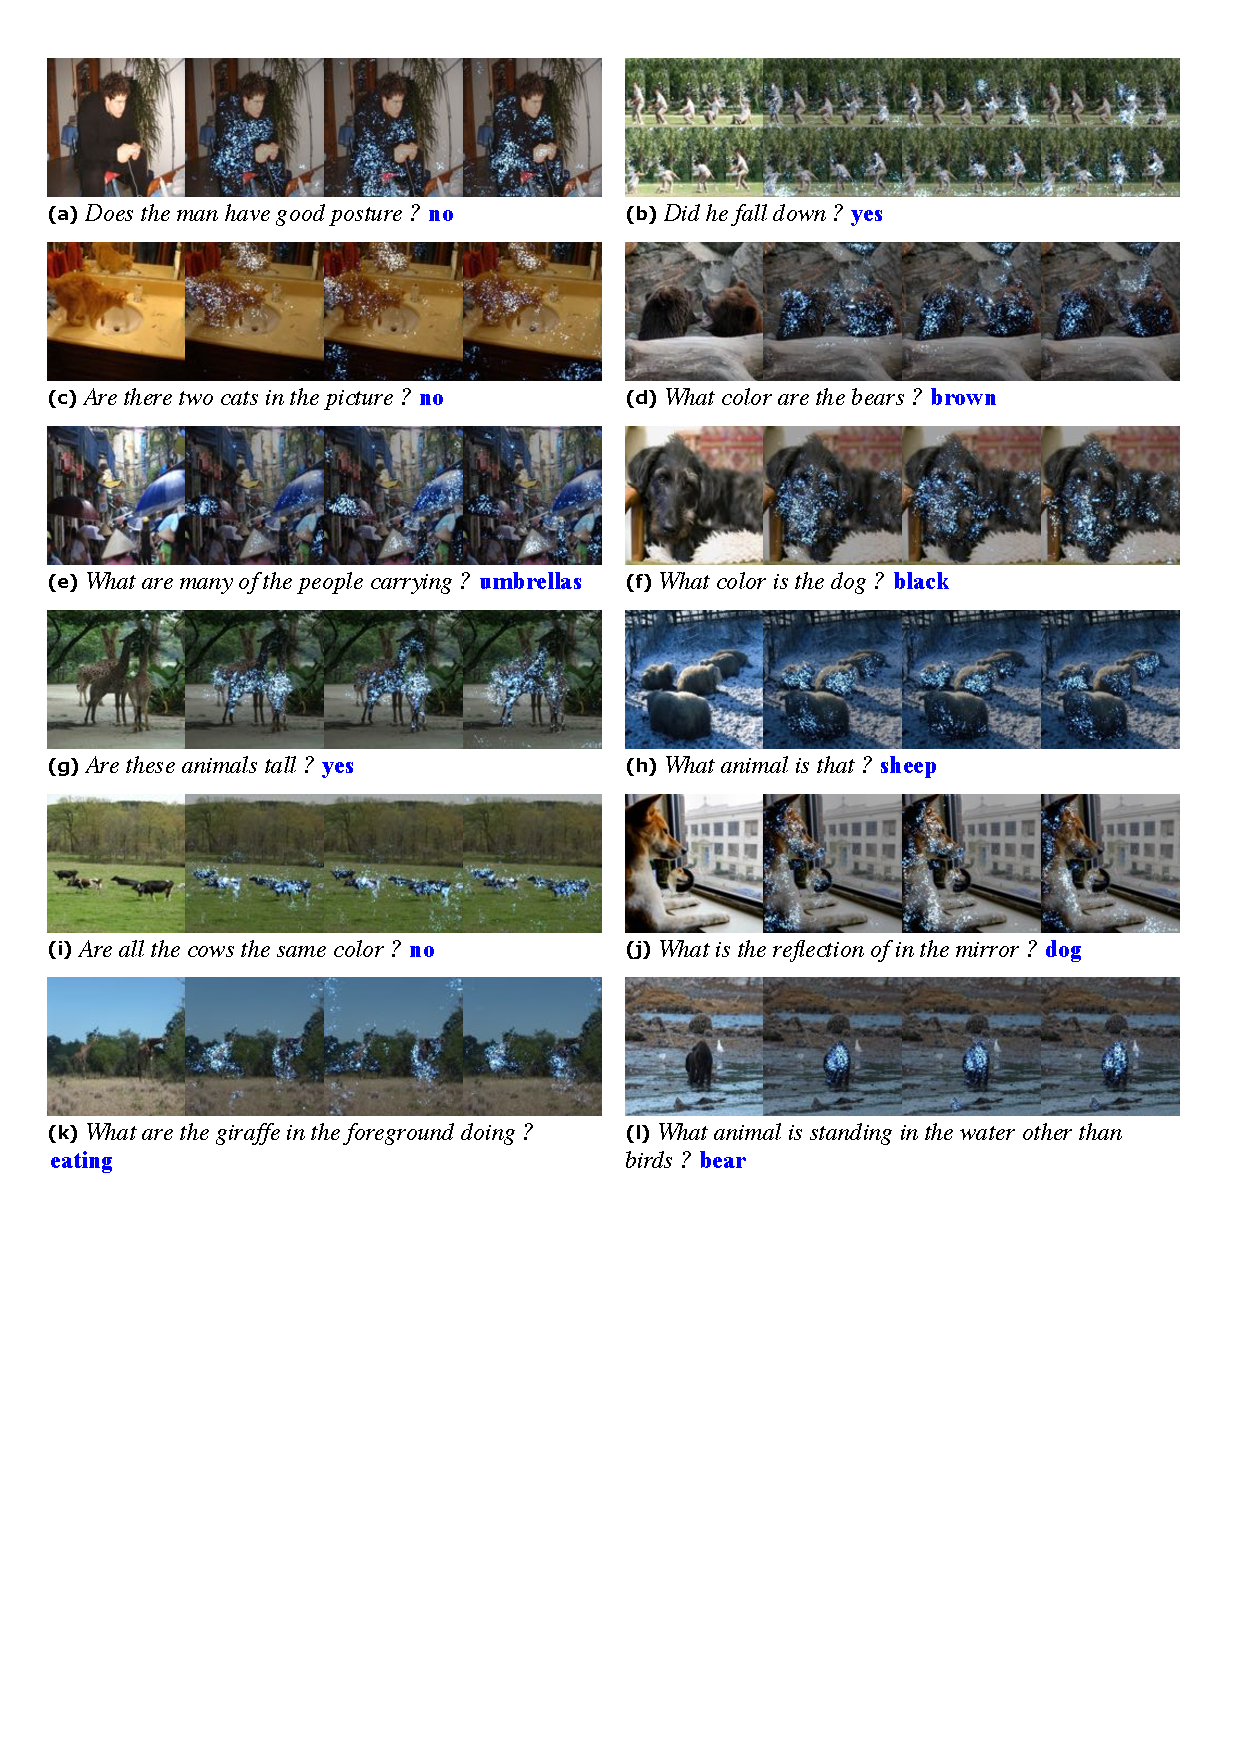
\includegraphics[width=\linewidth]{more_reduced}
\caption{More examples of Figure 4 in Section 5.2.}
\label{fig:more}
\end{figure} 

\newpage
\subsection{Comparative Analysis}

\begin{figure}[ht!]
\centering
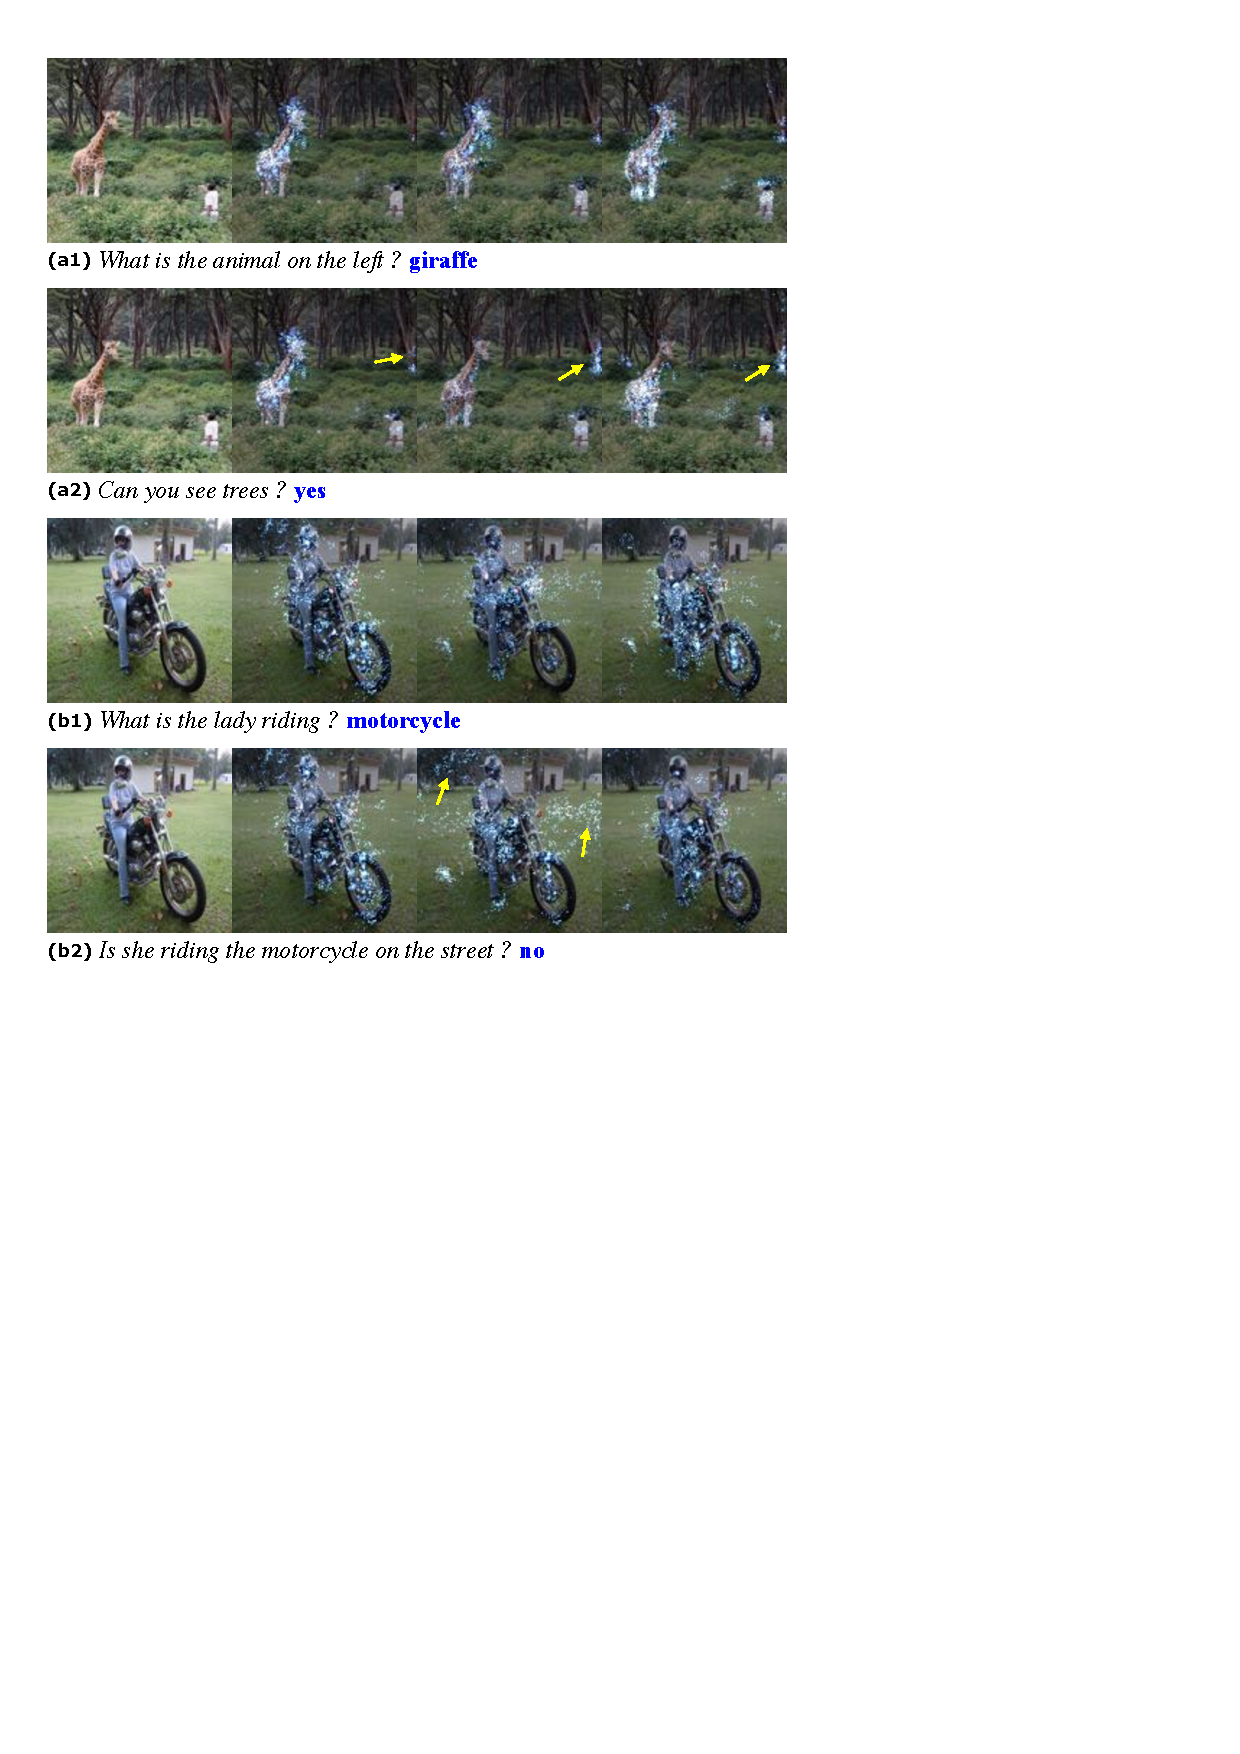
\includegraphics[width=.7\linewidth]{comp_reduced}
\caption{Comparative examples on the same image. (a1) and (a2) depict a giraffe (left) and a man pointing at the giraffe. MRN consistently highlights on the giraffe in (a1). However, the other question \textit{``Can you see trees?''} makes MRN less attentive to the giraffe, while a tree in the right of background is more focused in (a2). Similarily, the attention effect of (b2) is widely dispersed on background than (b1) in the middle of sequences, may be to recognize the site. However, the subtlety in comparative study is insufficient to objectively assess the results.}
\label{fig:comp}
\end{figure}

\newpage
\subsection{Failure Examples}

\begin{figure}[ht!]
\centering
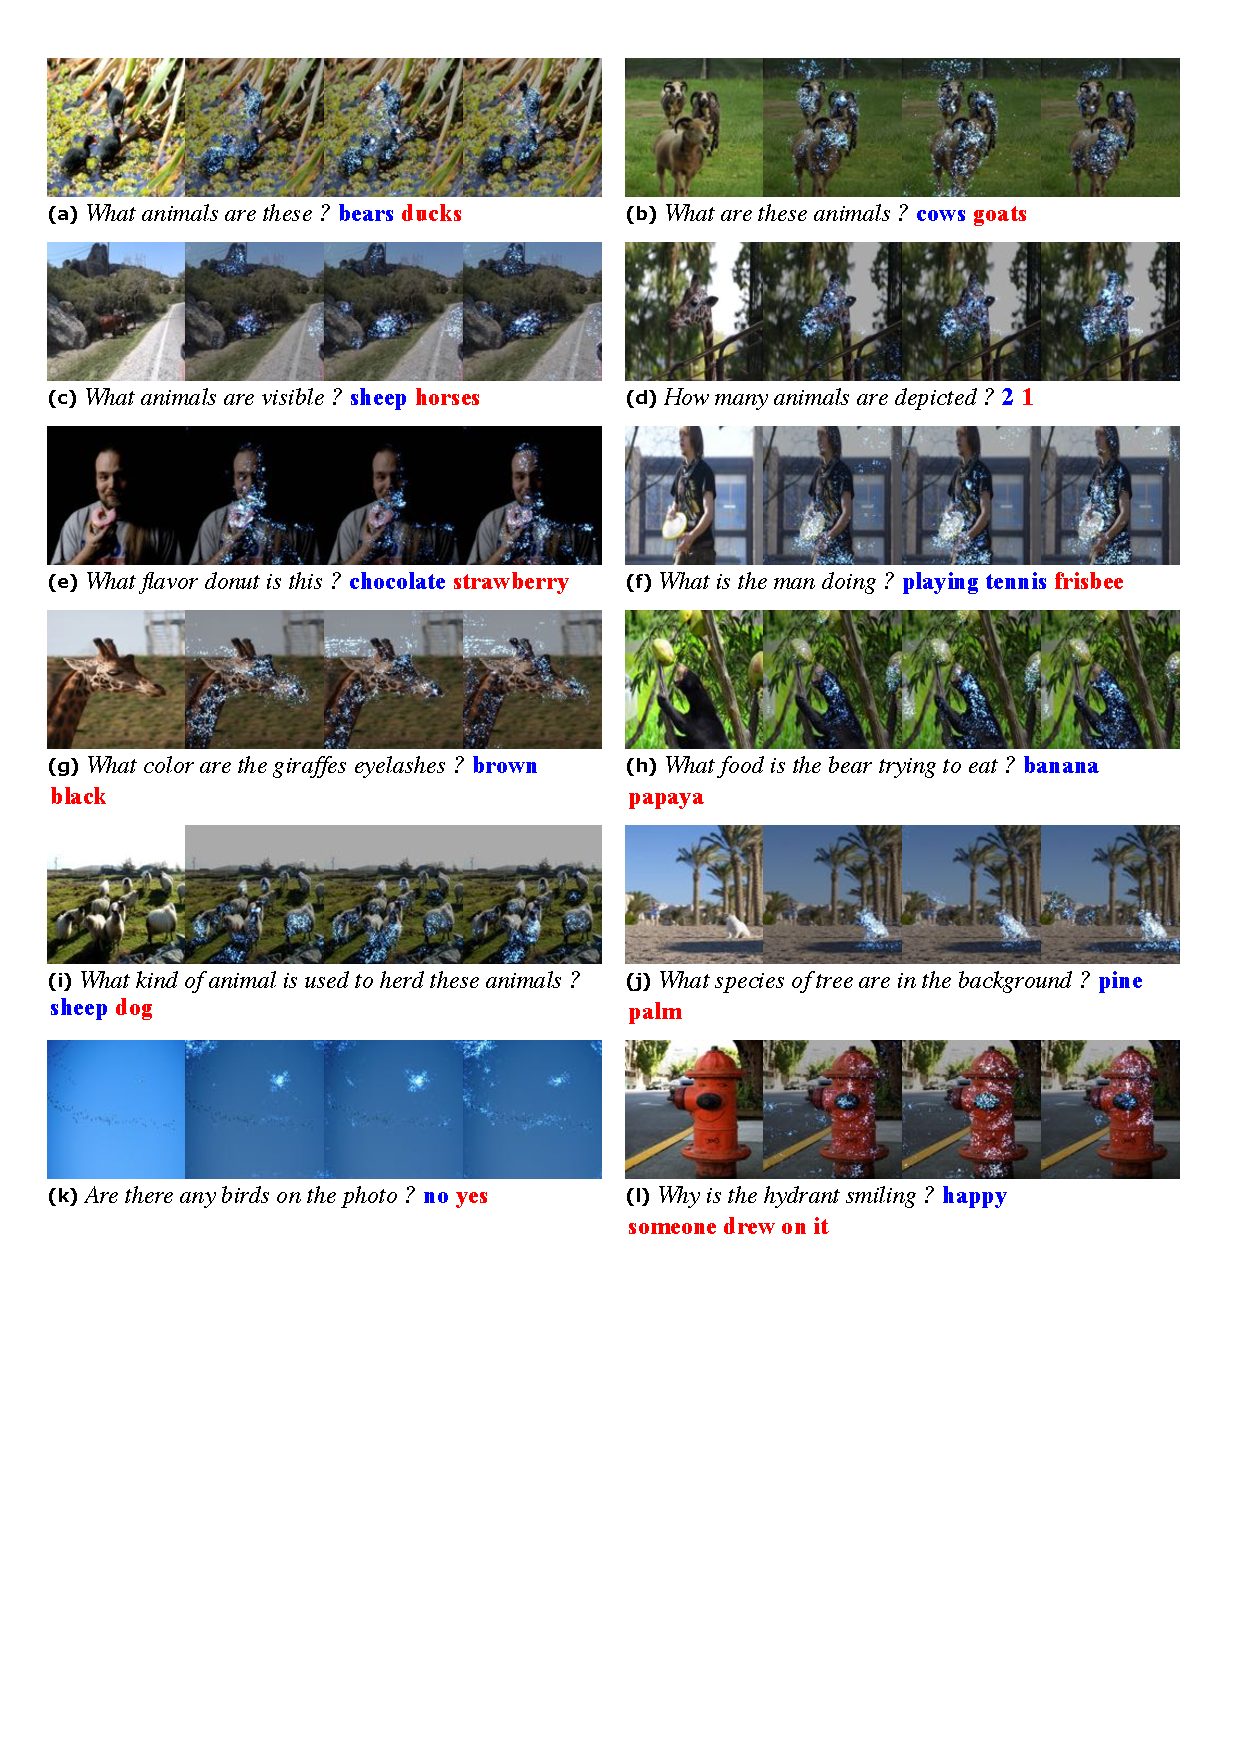
\includegraphics[width=\linewidth]{fail_reduced}
\caption{Failure Examples. Each question is followed by model prediction (blue) and answer (red). As mentioned in Section 5, MRN shows the weakness of counting in (d) and (k). Sometimes, the model finds objects regardless of the given question. In (j), even if a word \textit{cat} does not appear in the question, the cat in the image is surely attended. (i) shows the limitation of attentional mechanism, which needs an inference using world knowledge.}
\label{fig:more}
\end{figure}

